\chapter{Algorithmic Complexity}
\label{chapter:complexity}

The book embedding problem  without fixed page assignments  \probBookNormal is \NP-complete. For two pages
Bernhart~\cite{Bernhart79} showed that the problem is the same
as determining whether the graph is \emph{sub-hamiltonian}, \ie a subgraph of a planar
graph with a Hamiltonian cycle. This implies that \probBookNormal is \NP-complete by a result of Widgerson's~\cite{Widgerson82},
which states that the Hamiltonian circuit problem for maximal planar graphs is \NP-complete.

Since the two page case with fixed partitions is solvable in linear time~\cite{two-page-09},
we see that fixing the partitions significantly changes the book embedding problem. Is \probBook even
\NP-complete? We answer this question in the affirmative in the first
half of this chapter (\myref{section:np-complete}),
but, unfortunately, only for an unbounded number of pages. 

Thus, we know that \probBook is probably not efficiently solvable. In spite of that, we
want to test some specific instances in \myref{section:matchings}.
For this reason, in the second half of
this chapter~(\myref{section:sat}) we show how \probBook can be solved in super-polynomial time  by reducing it to \probThreeSat with some optimisations.
We chose the \probThreeSat problem since there are solvers for it that work well
on instances occurring in practice, even though \probThreeSat is \NP-complete.

\section{\textsc{Book-Embedding} is \NP-Complete}
\label{section:np-complete}

In this section we
construct a polynomial-time reduction from the \NP-complete problem \probBetween, defined below,
to \probBook, \ie we show that \probBook is \NP-complete. Therefore,
we cannot expect there to be an efficient algorithm for solving the general
book embedding problem.

Checking the book constraints for a pair of edges takes $\OO(1)$~time
and there are $\OO\bigl(\sum_{i} |E_i|^2\bigr)$ pairs to check.
Thus, checking the validity of a guessed book order takes polynomial
time and the book embedding problem must, therefore, be in~\NP.

We now give a polynomial time reduction from the problem \probBetween, which was shown to be \NP-complete by Opatrny~\cite{opatrny:79}, to \probBook and, thereby, show that \probBook itself is \NP-complete.

\newProb{\probBetween}{A finite set $M := \range{n}$ and a set of ordered triples $C \subseteq M^3$.}
{Is there a total ordering $<$ of $M$ such that either $a < b < c$ or $a > b > c$ occurs for all $(a, b, c) \in C$?}

The idea of the reduction is to map each triple to edges on two new pages that form a $C_4$, a cycle on 4~vertices. By
the following lemma, these two pages exactly represent the betweenness constraint.

\begin{figure}[\placement]\centering
    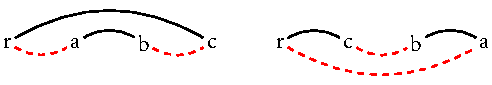
\includegraphics{figures/t_np_c4}
    \caption[Drawings of $C_4$]{The two drawings of a $C_4$ starting at $r$}
    \label{figure:np-c4}
\end{figure}

\begin{lemma}
\label{lemma:np-c4}
Let $V := \{r, a, b, c\}$, $E_1 := \bigl\{\{r, a\},\{b, c\}\bigr\}$ and $E_2 := \bigl\{\{a, b\}, \{r, c\}\bigr\}$. Then
$r < a < b < c$ and $r < c < b < a$, depicted in \myref{figure:np-c4}, are the only valid book embeddings of $E_1$ and $E_2$ with 
$r$ as first vertex.
\end{lemma}
\begin{myproof}
Let $<$ be a valid book order on $V$.
By \myref{lemma:constraints} the two pages yield the constraints $r < b < a \Leftrightarrow r < c < a$
and $r < a < c \Leftrightarrow r < b < c$. Since $r$ is the smallest element of $<$, this
is the same as $b < a \Leftrightarrow c < a \Leftrightarrow c < b$, \ie only the two cases $r < a < b < c$ and
$r < c < b < a$ remain.
\end{myproof}

Now let's do the formal reduction.

\begin{theorem}
\label{lemma:np-hard}
There is a polynomial time reduction from \probBetween to \probBook. Thus,
\probBook is \NP-complete.
\end{theorem}
\begin{myproof}
Let $I := (M, C)$ be a betweenness instance. 

Construct a book embedding instance $f(I) := \bigl(V, \bigcup_{t \in C} \left(E_{t,1} \cup E_{t,2}\right)\bigr)$ as follows.
Take $V := M\,\cup\,\{r\}$ as vertex set where $r \not\in M$ is a new symbol. For each triple $\tau~=~(a, b, c) \in C$ introduce
two new pages $E_{\tau, 1} := \bigl\{\{r, a\}, \{b, c\}\bigr\}$ and $E_{\tau, 2} := \bigl\{\{a, b\},\{r, d\}\bigr\}$. The instance $f(I)$ can obviously 
be computed in polynomial time.

Now show that $I$ is a positive instance if and only $f(I)$ is one.\nopagebreak
\begin{itemize}
\item[``$\Rightarrow$''] Let $I$ be a positive instance of \probBetween with valid total order $<$. Extend~$<$ to $V$ via
$r < k$ for all $k \in M$. For each triple $(a, b, c) \in C$ we have $r < a < b < c$ or $r < c < b < a$, \ie $<$ yields
a valid embedding of the pages by \myref{lemma:np-c4}. Thus, $<$ is a correct solution of $f(I)$.

\item[``$\Leftarrow$''] Let $f(I)$ be a positive instance of \probBook with valid total order~$<$. By \myref{lemma:symmetry} we
can assume  without loss
of generality that~$<$ is rotated such that $r$ is its smallest element. Then we have the situation of \myref{lemma:np-c4} for each triple $\tau = (a, b, c) \in C$ with
the pages~$E_{\tau,1}$ and $E_{\tau,2}$, \ie $a < b < c$ or $c < b < a$. Therefore, the order~$<$ restricted to $M$ is indeed a valid solution of $I$.\qedhere
\end{itemize}
\end{myproof}

We conclude that \probBook is \NP-complete. The reduction of
\myref{lemma:np-hard} gives us even more. The pages it creates are
matchings, \ie even the special case \probNotMatching of book embedding where the
edges on each page form a matching remains \NP-complete.

\newProb{\probNotMatching}{A vertex set $V$ and matchings $E_1, \dotsc, E_k \subseteq \binom{V}{2}$}%
{Is there a book embedding of $(V, E_1), \dotsc, (V, E_k)$?}

We do not know how complex the problem is when the edges on the pages form perfect matchings. This
special case is considered in more detail in \myref{section:matchings}.
%\begin{theorem}
%\label{theorem:np-complete}
%\probBook is \NP-complete.
%\end{theorem}
%\begin{myproof}
%Follows immediately from \myref{lemma:np-hard}.
%\end{myproof}
\section{Reduction to \probThreeSat}
\label{section:sat}

In the previous section we saw that~\probBook is \NP-complete.
This implies that we cannot expect to solve a general book embedding instance in polynomial time. 
But we still want to be able to check some instances, \eg to find counterexamples in special
cases as in \myref{section:matchings}. We, therefore, make it the goal
of this section to give a super-polynomial time algorithm for deciding book embeddability.

In order to achieve this, we express \probBook as a satisfiability problem of a Boolean formula.
The translation immediately yields a Boolean formula in 3-\CNF. That is,
the formula is a conjunction of disjunctions of literals (positive or negative variables) and each
disjunction contains at most~3 literals. The problem of deciding satisfiability for
these Boolean formulae is called~\probThreeSat and has been studied extensively.

\newProb{\probThreeSat}{A 3-\CNF Boolean formula \bool{f}.}{Is~\bool{f} satisfiable?}

Although \probThreeSat was the first problem to be proven \NP-complete~\cite{Cook71}, there
are \SAT-solvers that handle many instances occurring in practice in reasonable times. One that
has scored well in several contests is~\mytt{minisat}~\cite{minisat03}. We use it to 
check the resulting formulae for some instances in \myref{section:matchings}.

Now we derive the translation of the total order formulation of~\probBook from \myref{lemma:constraints}
into a Boolean formula. Let $\bigl((V, E_1),\dotsc, (V, E_k)\bigr)$ be the book embedding 
instance and label the vertices $V = \range{n}$ without loss of generality. 

We have to express the total order~$<$ as a set of Boolean variables. 
It is natural to introduce a variable
\bool{v(i, j)} for the statement $i < j$ for all $i, j \in V$. 

Then we have to build a 3-\CNF formula that rephrases the stipulation that~$<$ is a
strict total order and that the book constraints are fulfilled. We can achieve this by forming the conjunction of the following formulae.

\paragraph{Strict total order}

That~$<$ is a strict total order means, by definition, that it is asymmetric, irreflexive, transitive
and total:

\begin{description}
\item[irreflexive] For each vertex~$i \in V$ the formula~$i < i$ is false. 
We get~$\lnot v(i, i)$. (n~clauses)
\item[asymmetric and total] For each unordered pair of distinct vertices~$i, j \in V$ exactly one
of~$i < j$ or~$j < i$ is true. We get~$v(i,j) \xor v(j,i) \equiv \bigl(v(i,j) \lor v(j,i)\bigr) \land \bigl(\lnot v(i,j) \lor \lnot v(j,i)\bigr)$. (two~clauses for each of the $\binom{n}{2}$~unordered pairs)
\item[transitive] For each triple~$i, j, k \in V$ of vertices, if~$i < j$ and $j < k$ are
true, then also~$i < k$. We get~$\bigl(v(i, j) \land v(j, k)\bigr) \Rightarrow v(i, k) \equiv \lnot v(i, j)
\lor \lnot v(j, k) \lor v(i, k)$. (one clause for each of the $n(n-1)(n-2)$~ordered triples of
distinct vertices)
\end{description}

\paragraph{Book constraints}

For each unordered pair of different edges~$e_1 := \{a, b\}, e_2 := \{c, d\} \in E_i$, we have to take the book 
constraint from \myref{def:book-constraint} into account. The constraint says exactly that~$c$ is between~$a$
and~$b$ if and only if~$d$ is between~$a$ and~$b$ as well as that~$a$ is between~$c$ and~$d$
if and only if~$b$ is between~$c$ and~$d$. 

% We rephrase it as follows: If one
%vertex of one of the two edges lies between the vertices of the other, then the other 
%vertex of the first edge also lies between the vertices of the second. Furthermore, we have to
%consider all possible orders of $a$~and~$b$ respectively $c$~and~$d$.

That is, if we choose one of the edges $e_1$ or~$e_2$ as edge~$e_O := \{w, x\}$ and the other as
edge~$e_I := \{y, z\}$, we get the following equivalence:
\[
%\bigwedge_{\substack{e_O, e_I \in \{e_1, e_2\}\\e_I \neq e_O, e_I =: \{y, z\}}} \bigwedge_{\substack{w, %x \in e_O\\w \neq x}} \Bigl(v(w, y) \land v(y, x) \Leftrightarrow v(w, z) \land v(z, x)\Bigr) 
\bigl(v(w, y) \land v(y, x) \Leftrightarrow v(w, z) \land v(z, x)\bigr) \tag{1}
\]
Exchanging the vertices $y$ and~$z$ does not change the resulting clauses, while
exchanging the vertices $w$ and~$x$ does. Thus, there are two choices to make. Firstly,
which of $e_1$ and~$e_2$ gets the name~$e_O$ and which gets the
name~$e_I$ (two possibilities). Secondly, which incident vertex of the edge~$e_O$ gets the
name~$w$ and which gets the name~$x$ (two possibilities).

Since the formula~(1) is equivalent to the \CNF-formula $\bigl(\lnot v(w, y) \lor \lnot v(y, x) \lor v(w, z)\bigr) \land\allowbreak\bigl(\lnot v(w, y) \lor \lnot v(y, x) \lor v(z, x)\bigr) \land \bigl(\lnot v(w, z) \lor \lnot v(z, x) \lor v(w, y)\bigr) \land \bigl(\lnot v(w, z) \lor \lnot v(z, x) \lor v(y, x)\bigr)$, we get $\text{2}\cdot \text{2} \cdot \text{4} = \text{16}$ clauses for each of
the $\sum_{i=1}^{k} \binom{|E_i|}{2}$ unordered pairs of edges.

We actually do not need the clauses for both choices of~$e_O$. Once the \SAT-formulae for one choice have been added, the constraints for the other choice immediately follow.

We now show this observation. Let $e_1 := \{a, b\}, e_2 := \{c, d\}$ be edges and
assume we have the \SAT-formulae of type~(1) with $e_O = e_1$ as well as the \SAT-formulae for the asymmetry and totality. 
We now show $v(c, a) \land v(a, d) \Rightarrow v(c, b) \land v(b, d)$. The other
instances of~(1) with~$e_O = e_2$ can be proven analogously. 

Assume that $v(c, a) \land v(a, d)$ is true.
If~$v(d, b)$ is true, we can infer $v(a, c)$ by $v(a, d) \land v(d, b) \Leftrightarrow
v(a, c) \land v(c, b)$ (the formula~(1) with $e_O = \{a, b\}$, $w = a$ and $x = b$) which contradicts $v(c, a)$ because of the asymmetry constraint. 
That is, $v(b, d)$~must be true by the asymmetry and totality.
In the
same manner we can show~$v(c, b)$. Thus, the assumption implies $v(c, b) \land v(b, d)$,
as desired.

This small optimisation saves half of the clauses,
\ie we only need eight~clauses for each pair of edges.

\paragraph{Fixed minimum}

From \myref{lemma:symmetry} we know that cyclic shifts preserve the validity of~$<$.
To help the \SAT-solver, we can, therefore, assume that~$1$ is the
smallest vertex and add the clauses~$v(1, j)$ for all $j \in V$ with $j \neq 1$. They
comprise another~$n-1$ clauses.

\begin{table}[tb]
\centering

\resizebox{\textwidth}{!}{
\begin{tabular}{lll}

\textbf{Axiom} & \textbf{3-\CNF formula} & \textbf{Number of clauses}\\
\toprule
Irreflexive          & $\lnot v(i, i)$ & $n$ \\
\midrule
Asymmetric and total & $\bigl(v(i,j) \lor v(j,i)\bigr) \land \bigl(\lnot v(i,j) \lor \lnot v(j,i)\bigr)$ & $2\binom{n}{2}$\\
                     & for all distinct unordered pairs $i, j \in V$ \\
\midrule
Transitive           & $\lnot v(i, j) \lor \lnot v(j, k) \lor v(i, k)$ & $n(n-1)(n-2)$\\ 
                     & for all ordered triples $i, j, k \in V$ where\\
                     & $i$, $j$~and $k$ are pairwise distinct\\
\midrule
Book embedding       & $\bigl(\lnot v(w, y) \lor \lnot v(y, x) \lor v(w, z)\bigr)$ & $16\cdot\sum_{i=1}^{k} \binom{|E_i|}{2}$\\
                     & $\land \bigl(\lnot v(w, y) \lor \lnot v(y, x) \lor v(z, x)\bigr)$ \\
                     & $\land \bigl(\lnot v(w, z) \lor \lnot v(z, x) \lor v(w, y)\bigr)$ \\
                     & $\land \bigl(\lnot v(w, z) \lor \lnot v(z, x) \lor v(y, x)\bigr)$ \\
                     & for all distinct $e_O = \{w, x\}$, \\
                     & $e_I = \{y, z\} \in E_i$ and all $i \in \range{k}$ \\
                     & where it matters which edge is\\
                     & assigned to $e_O$ and which to $e_I$\\
\midrule
Book embedding       & $\bigl(\lnot v(w, y) \lor \lnot v(y, x) \lor v(w, z)\bigr)$ & $8\cdot\sum_{i=1}^{k} \binom{|E_i|}{2}$\\
(optimised)          & $\land \bigl(\lnot v(w, y) \lor \lnot v(y, x) \lor v(z, x)\bigr)$ \\
                     & $\land \bigl(\lnot v(w, z) \lor \lnot v(z, x) \lor v(w, y)\bigr)$ \\
                     & $\land \bigl(\lnot v(w, z) \lor \lnot v(z, x) \lor v(y, x)\bigr)$ \\
                     & for all distinct $e_O = \{w, x\}$,\\
                     & $e_I = \{y, z\} \in E_i$ and all $i \in \range{k}$\\
                     & where it does not matter which edge is\\
                     & assigned to $e_O$ and which to $e_I$\\
\midrule
Fixed minimum         & $v(1, j)$ for all $j \in \bigl(V \setminus \{1\}\bigr)$ & $n - 1$\\
\bottomrule
\end{tabular}}

\caption[\CNF translation of \probBook]{The 3-\CNF formulae corresponding to \probBook}
\label{table:sat}
\end{table}

The clauses we get are summarised in \myref{table:sat}. They
provide us with a polynomial-time reduction from~$\probBook$ to~$\probThreeSat$.
The number of edges $|E_i|$ is linear in $|V|$ for all~$i \in \range{k}$ since~$(V, E_i)$ is an outerplanar graph.
Thus, we get~$\OO\bigl(|V|^3 + k|V|^2\bigr)$ clauses.

\begin{theorem}
Let~$I := (V, E_1, \dotsc, E_k)$ be a~$\probBook$ instance. There is a $\OO\bigl(|V|^3 + k|V|^2\bigr)$~time reduction
to an equivalent $\probThreeSat$ instance with~$\OO\bigl(|V|^3 + k|V|^2\bigr)$ clauses.
%$\probBook \leq_P \probThreeSat$
\end{theorem}
%\begin{myproof}
%The translated constraints in \myref{table:sat} which we can write down
%in polynomial time directly express the book embedding problem as 3-\prob{cnf} formula.
%\end{myproof}

%%% Local Variables: 
%%% mode: latex
%%% TeX-master: "thesis"
%%% End: 
